\documentclass[11pt,letterpaper]{article}
\usepackage[utf8]{inputenc}
\usepackage[T1]{fontenc}
\usepackage[spanish]{babel}
\usepackage[margin=2.25cm]{geometry}
\usepackage{graphicx}
\usepackage{amsmath}
\usepackage{booktabs}
\usepackage{caption}
\usepackage{float}
\usepackage{hyperref}
\usepackage{xcolor}
\usepackage{enumitem}
\usepackage{array}
\hypersetup{colorlinks=true,linkcolor=blue!45!black,citecolor=blue!45!black,urlcolor=blue!45!black}
\setlength{\parindent}{0pt}
\setlength{\parskip}{4pt}
\setlist[itemize]{leftmargin=1.3em,itemsep=1pt,topsep=2pt}
\captionsetup{font=small,labelfont=bf}

\begin{document}

\begin{titlepage}
\centering
\includegraphics[width=.42\textwidth]{ucb-logo.png}\\[.2cm]
{\large UNIVERSIDAD CATÓLICA BOLIVIANA ``SAN PABLO''}\\[0.1cm]
{\large SEDE SANTA CRUZ}\\[0.8cm]
{\large MAESTRÍA EN CIENCIA DE DATOS E INTELIGENCIA ARTIFICIAL APLICADA}\\[0.35cm]
{\large MCI-509 PROCESAMIENTO DE IMÁGENES Y VISIÓN COMPUTACIONAL}\\[0.9cm]
\rule{\textwidth}{0.4pt}\\[0.45cm]
{\LARGE\bfseries Project AmarketBoundingBoxes: detección multiproducto e identificación visual de SKU}\\[0.45cm]
\rule{\textwidth}{0.4pt}\\[0.9cm]
{\large\textbf{Integrantes del equipo:}}\\[0.25cm]
{\large Guillermo Carvajal Vaca\\Montserrat Barba\\Andrés Poiche\\Pablo Linares\\}
\vfill
{\large Santa Cruz de la Sierra, Bolivia}\\
{\large 23 de agosto de 2026}
\end{titlepage}

% IMPORTANTE: esta sección se cerrará cuando exista evidencia de FASE 6
% o cuando el coordinador confirme que la identificación queda solo en piloto.
\section*{Resumen}
\emph{Sección reservada para el cierre del informe. El resumen final de 150--200 palabras se redactará cuando se conozca el estado definitivo de la evaluación de identificación (FASE 6).}

\section{Introducción y motivación}
El proyecto aborda un único problema end-to-end: dada una escena tipo caja o supermercado con varios productos, localizar cada producto visible e intentar asociarlo con su identidad de catálogo (SKU y nombre). El reto combina dos niveles que forman parte de la misma solución: localizar correctamente cada instancia y distinguir después variantes visualmente muy parecidas, por ejemplo presentaciones o tonos de una misma familia.

Este tipo de sistema se aproxima a tareas de asistencia en caja, inventario visual y verificación de productos. Una solución útil no puede interpretar una caja correctamente detectada como una identidad correctamente reconocida; por ello la arquitectura conserva señales separadas dentro del mismo pipeline. YOLO11n aporta la localización y su \emph{yolo\_confidence}; sobre cada recorte detectado, el retrieval visual SIFT intenta recuperar la referencia de catálogo. La similitud de SIFT no se presenta como probabilidad calibrada de identidad ni se mezcla con la confianza del detector.

La motivación del trabajo es construir una línea base reproducible sobre datos propios de AMARKET que permita evaluar el flujo completo y, al mismo tiempo, identificar con honestidad cuál componente limita el desempeño del sistema.

\section{Datos}
El conjunto real proviene de imágenes públicas de productos del catálogo de AMARKET. Se conservaron 655 imágenes reales y se utilizó semilla 42 para la partición: 459 imágenes de entrenamiento, 98 de validación y 98 de test. La tarea YOLO es monoclase, con \texttt{class\_id=0} y \texttt{class\_name=product}; SKU y nombre se mantienen como metadatos y no como clases YOLO. Los conjuntos de validación y test contienen exclusivamente imágenes reales.

\begin{table}[H]
\centering
\small
\caption{Composición efectivamente utilizada en el experimento.}
\begin{tabular}{lrrl}
\toprule
Conjunto & Imágenes & Objetos/placements & Observación \\
\midrule
Train real & 459 & 459 & Imágenes reales aisladas \\
Train sintético & 197 & 481 & Todas \texttt{difficulty=basic} \\
Train combinado & 656 & -- & 459 reales + 197 sintéticas \\
Validación & 98 & 98 & Solo imágenes reales \\
Test & 98 & 98 & Solo imágenes reales, bloqueado \\
\bottomrule
\end{tabular}
\end{table}

La generación sintética planificó originalmente 655 escenas y 3287 placements. Esa corrida no terminó y falló en \texttt{SYN\_0198}; por tanto, 655/3287 describen únicamente el diseño planificado. El entrenamiento que se documenta utilizó realmente 197 escenas sintéticas y 481 placements, combinadas con las 459 imágenes reales de train para un total de 656 imágenes de entrenamiento.

Todas las escenas sintéticas disponibles para esta corrida son de dificultad \texttt{basic}. Esto limita la representación de clutter, oclusiones, iluminación variable, reflejos y fondos complejos propios de escenarios reales. No se identificó una licencia explícita del catálogo que autorice redistribuir las imágenes como dataset. En consecuencia, el conjunto se conserva en Drive privado para uso académico y no se redistribuye públicamente. La procedencia del catálogo es AMARKET (\url{https://amarket.com.bo/}); documentar la fuente no equivale a atribuir una licencia inexistente.

\section{Metodología y arquitectura}
\textbf{Pipeline integrado.} La solución se modela como una única arquitectura de dos etapas encadenadas. Primero, YOLO11n localiza cada producto mediante bounding boxes. Después, cada recorte detectado se entrega al módulo de retrieval visual SIFT, que intenta asociarlo con una referencia de catálogo y recuperar SKU y nombre. Estas etapas no constituyen dos entregas independientes: juntas forman el flujo de inferencia del proyecto.

\textbf{Composición sintética.} Las imágenes reales de entrenamiento se complementaron con escenas sintéticas multiproducto. Para mantener trazabilidad, solo se consideran las 197 escenas que realmente estaban disponibles y fueron utilizadas; no se atribuye al experimento la corrida planificada de 655 escenas que no finalizó.

\textbf{Detector.} Se utilizó YOLO11n preentrenado y adaptado a una única clase. Se ejecutaron dos corridas comparables, B0 y T1, ambas durante 40 épocas. T1 registra \texttt{imgsz=512}, \texttt{batch=8}, semilla 42 y entrenamiento determinista. Con \texttt{optimizer=auto}, Ultralytics resolvió AdamW con learning rate inicial 0.002, momentum 0.9 y \texttt{weight\_decay=0.0005}. El criterio de selección se fijó sobre validación: mayor mAP50-95, sin utilizar test para escoger hiperparámetros.

\textbf{Identificación.} SIFT calcula descriptores locales de cada recorte y los compara con las referencias de catálogo. El resultado de retrieval se evalúa mediante Top-1 y Top-5. La puntuación mostrada junto al nombre en las imágenes anotadas corresponde a \emph{yolo\_confidence} de la caja, no a una probabilidad de que la identidad recuperada sea correcta. La similitud SIFT debe interpretarse y reportarse por separado.

\subsection*{Reproducibilidad}
La semilla contractual es 42 y los splits reales permanecen definidos. La evidencia entregada por el coordinador registra que \texttt{notebooks/inferencia\_cpu.ipynb} fue ejecutado mediante \texttt{nbconvert --execute}, equivalente a Restart \& Run All, con CPU forzado, artefactos reales, sin rutas absolutas hardcodeadas y exit code 0. Este informe atribuye esa ejecución a la evidencia del coordinador; no afirma que se haya ejecutado nuevamente en la máquina usada para redactar el documento.

El test del detector permaneció bloqueado hasta completar la selección del modelo. T1 se seleccionó por validación antes de abrir el test y no se realizó tuning posterior utilizando los resultados de test.

\section{Resultados observados hasta el cierre parcial}
\subsection*{Detector}
B0 y T1 completaron las 40 épocas planificadas. El mayor mAP50-95 observado en validación fue 0.98679 para B0 y 0.99093 para T1; por ello T1 fue seleccionado. Después de congelar esa selección se ejecutó una única evaluación sobre el test real: Precision=0.9857, Recall=1.0000, mAP50=0.9941 y mAP50-95=0.9715. No hubo tuning posterior mirando test.

\begin{table}[H]
\centering
\small
\caption{Resultados observados del detector.}
\begin{tabular}{lcccc}
\toprule
Evaluación & Precision & Recall & mAP50 & mAP50-95 \\
\midrule
B0, mejor validación & -- & -- & -- & 0.98679 \\
T1, mejor validación & -- & -- & -- & \textbf{0.99093} \\
T1, test real & 0.9857 & 1.0000 & 0.9941 & 0.9715 \\
\bottomrule
\end{tabular}
\end{table}

\begin{figure}[H]
\centering
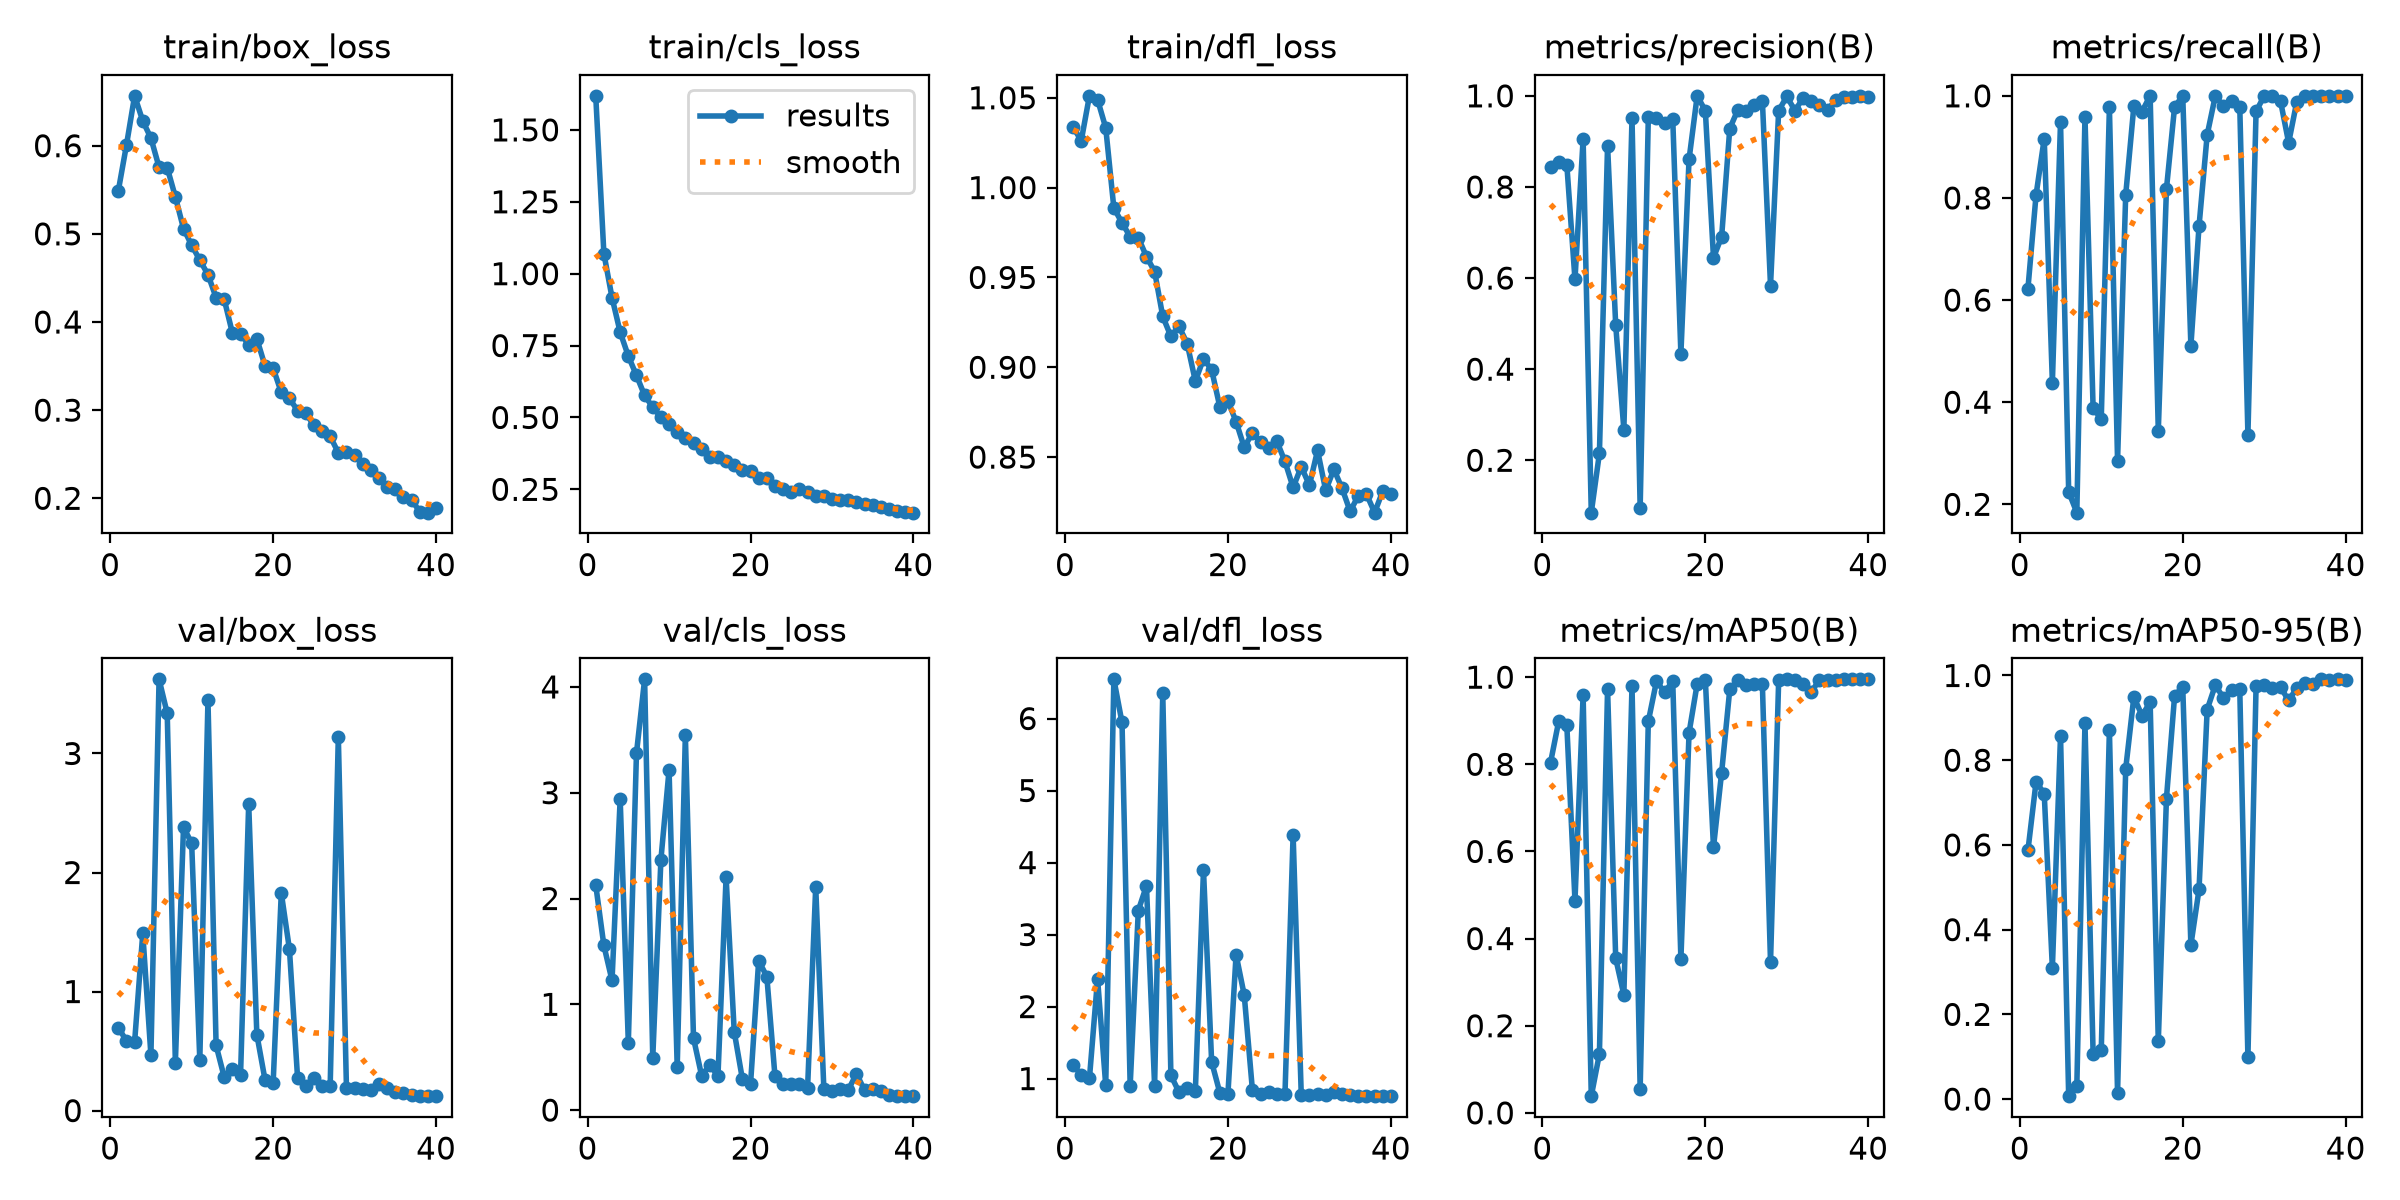
\includegraphics[width=.91\textwidth]{figuras/t1_train_val_results.png}
\caption{Artefacto real de entrenamiento de T1 durante 40 épocas. Incluye pérdidas de train/val y métricas de validación; no fue regenerado para el informe.}
\label{fig:t1curves}
\end{figure}

\subsection*{Identificación: evidencia disponible, no cierre final}
Existe una validación piloto gobernada de 10 escenas y 20 productos. En ella SIFT obtuvo Top-1 accuracy=35\% y Top-5 accuracy=50\%. Estas cifras se documentan únicamente como evidencia piloto y no se presentan como evaluación final completa del módulo de identificación.

La evaluación end-to-end prevista sobre las 197 escenas y 481 productos se encuentra en ejecución fuera de esta máquina. Mientras no exista evidencia de finalización con exit code 0, el informe no asignará a esa evaluación estado PASS, FAIL ni métrica final. Si FASE 6 concluye antes del cierre, su métrica observada reemplazará este estado provisional en el PDF final. Si no concluye, el informe final declarará explícitamente que la identificación quedó evaluada solo mediante validación piloto.

\begin{figure}[H]
\centering
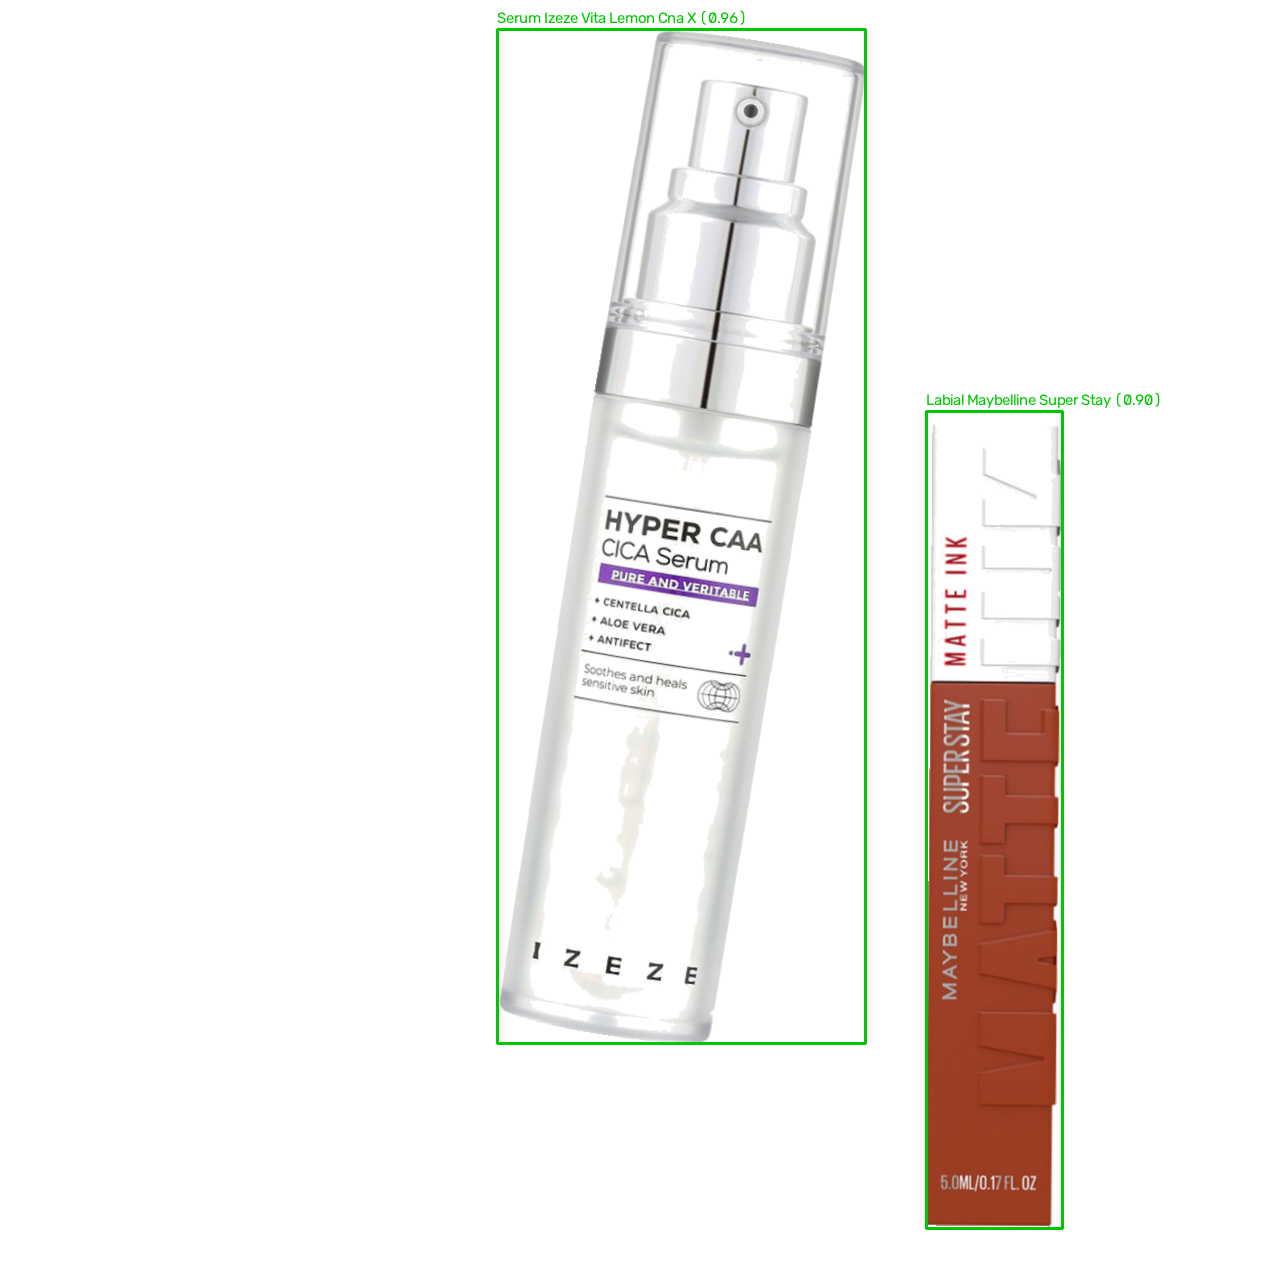
\includegraphics[width=.72\textwidth]{figuras/syn0001_identity_error.png}
\caption{\texttt{SYN\_0001}: las dos cajas están correctamente localizadas, pero las identidades recuperadas no coinciden exactamente con el ground truth. El sérum real es Izeze Hyper Caa Cica (SKU 8809686120260) y se recupera Izeze Vita Lemon Cna (SKU 8809686120338); el labial real es Maybelline tono 505 Entertainer (SKU 041554098228) y se recupera tono 500 Insider (SKU 041554098211). Los valores 0.96 y 0.90 son confianza YOLO de detección, no confianza de identidad.}
\label{fig:synerror}
\end{figure}

\section{Discusión y limitaciones}
La evidencia observada sugiere que la localización de productos está bien resuelta dentro del dominio evaluado, mientras que la identificación exacta de variantes sigue siendo el componente más sensible. Esto debe interpretarse como desempeño de componentes dentro de un único pipeline, no como dos entregas separadas. Una caja puede tener alta confianza YOLO y aun así recuperar una variante o SKU incorrecto.

Las limitaciones principales son cuatro. Primero, el entrenamiento sintético realmente usado cubre solo 197 escenas de dificultad básica y no representa de forma suficiente clutter, oclusiones, reflejos ni condiciones de iluminación complejas. Segundo, las imágenes reales de origen son principalmente productos aislados, por lo que existe una brecha respecto de escenas reales multiproducto. Tercero, SIFT depende de textura y keypoints locales, lo que dificulta separar productos de una misma familia cuando los cambios están concentrados en texto pequeño, tonos o detalles del empaque. Cuarto, la evaluación completa de identificación aún no dispone de evidencia de finalización; por ello 35\% Top-1 y 50\% Top-5 deben leerse exclusivamente como validación piloto de 20 productos.

No se identificó una licencia explícita que autorice redistribuir el catálogo como dataset, por lo que los datos permanecen privados para uso académico. Asimismo, no se afirma una garantía absoluta de ausencia de fuga más allá del protocolo de partición aplicado. El test permaneció bloqueado hasta seleccionar T1 y no se reutilizó para ajustar el modelo.

\section{Trabajo futuro}
\begin{itemize}
\item Sustituir o complementar SIFT con embeddings visuales preentrenados y congelar un protocolo Top-$k$ comparable.
\item Incorporar más referencias por SKU y por variante, especialmente tonos y presentaciones muy similares.
\item Construir escenas reales multiproducto con mayor clutter, iluminación y oclusión manteniendo splits independientes.
\item Optimizar y cachear descriptores o embeddings del catálogo para reducir el costo de retrieval sin alterar el protocolo de evaluación.
\end{itemize}

% IMPORTANTE: no cerrar esta sección hasta conocer el estado definitivo de FASE 6.
\section{Conclusiones}
\emph{Sección reservada para el cierre final. Las conclusiones se redactarán después de incorporar la métrica observada de FASE 6 si la evaluación completa finaliza; de lo contrario, declararán explícitamente que la identificación quedó evaluada únicamente mediante el piloto gobernado.}

\clearpage
\begin{thebibliography}{9}
\bibitem{ultralytics2024}
G. Jocher y J. Qiu. \textit{Ultralytics YOLO11}, 2024. Documentación oficial: \url{https://docs.ultralytics.com/models/yolo11}.

\bibitem{lowe2004}
D. G. Lowe. ``Distinctive Image Features from Scale-Invariant Keypoints''. \textit{International Journal of Computer Vision}, 60(2):91--110, 2004.

\bibitem{amarket}
AMARKET Bolivia. Catálogo público utilizado como fuente de imágenes de producto. \url{https://amarket.com.bo/}. No se identificó una licencia explícita que autorice su redistribución como dataset.
\end{thebibliography}

\end{document}
